\documentclass[1p]{elsarticle_modified}
%\bibliographystyle{elsarticle-num}

%\usepackage[colorlinks]{hyperref}
%\usepackage{abbrmath_seonhwa} %\Abb, \Ascr, \Acal ,\Abf, \Afrak
\usepackage{amsfonts}
\usepackage{amssymb}
\usepackage{amsmath}
\usepackage{amsthm}
\usepackage{scalefnt}
\usepackage{amsbsy}
\usepackage{kotex}
\usepackage{caption}
\usepackage{subfig}
\usepackage{color}
\usepackage{graphicx}
\usepackage{xcolor} %% white, black, red, green, blue, cyan, magenta, yellow
\usepackage{float}
\usepackage{setspace}
\usepackage{hyperref}

\usepackage{tikz}
\usetikzlibrary{arrows}

\usepackage{multirow}
\usepackage{array} % fixed length table
\usepackage{hhline}

%%%%%%%%%%%%%%%%%%%%%
\makeatletter
\renewcommand*\env@matrix[1][\arraystretch]{%
	\edef\arraystretch{#1}%
	\hskip -\arraycolsep
	\let\@ifnextchar\new@ifnextchar
	\array{*\c@MaxMatrixCols c}}
\makeatother %https://tex.stackexchange.com/questions/14071/how-can-i-increase-the-line-spacing-in-a-matrix
%%%%%%%%%%%%%%%

\usepackage[normalem]{ulem}

\newcommand{\msout}[1]{\ifmmode\text{\sout{\ensuremath{#1}}}\else\sout{#1}\fi}
%SOURCE: \msout is \stkout macro in https://tex.stackexchange.com/questions/20609/strikeout-in-math-mode

\newcommand{\cancel}[1]{
	\ifmmode
	{\color{red}\msout{#1}}
	\else
	{\color{red}\sout{#1}}
	\fi
}

\newcommand{\add}[1]{
	{\color{blue}\uwave{#1}}
}

\newcommand{\replace}[2]{
	\ifmmode
	{\color{red}\msout{#1}}{\color{blue}\uwave{#2}}
	\else
	{\color{red}\sout{#1}}{\color{blue}\uwave{#2}}
	\fi
}

\newcommand{\Sol}{\mathcal{S}} %segment
\newcommand{\D}{D} %diagram
\newcommand{\A}{\mathcal{A}} %arc


%%%%%%%%%%%%%%%%%%%%%%%%%%%%%5 test

\def\sl{\operatorname{\textup{SL}}(2,\Cbb)}
\def\psl{\operatorname{\textup{PSL}}(2,\Cbb)}
\def\quan{\mkern 1mu \triangleright \mkern 1mu}

\theoremstyle{definition}
\newtheorem{thm}{Theorem}[section]
\newtheorem{prop}[thm]{Proposition}
\newtheorem{lem}[thm]{Lemma}
\newtheorem{ques}[thm]{Question}
\newtheorem{cor}[thm]{Corollary}
\newtheorem{defn}[thm]{Definition}
\newtheorem{exam}[thm]{Example}
\newtheorem{rmk}[thm]{Remark}
\newtheorem{alg}[thm]{Algorithm}

\newcommand{\I}{\sqrt{-1}}
\begin{document}

%\begin{frontmatter}
%
%\title{Boundary parabolic representations of knots up to 8 crossings}
%
%%% Group authors per affiliation:
%\author{Yunhi Cho} 
%\address{Department of Mathematics, University of Seoul, Seoul, Korea}
%\ead{yhcho@uos.ac.kr}
%
%
%\author{Seonhwa Kim} %\fnref{s_kim}}
%\address{Center for Geometry and Physics, Institute for Basic Science, Pohang, 37673, Korea}
%\ead{ryeona17@ibs.re.kr}
%
%\author{Hyuk Kim}
%\address{Department of Mathematical Sciences, Seoul National University, Seoul 08826, Korea}
%\ead{hyukkim@snu.ac.kr}
%
%\author{Seokbeom Yoon}
%\address{Department of Mathematical Sciences, Seoul National University, Seoul, 08826,  Korea}
%\ead{sbyoon15@snu.ac.kr}
%
%\begin{abstract}
%We find all boundary parabolic representation of knots up to 8 crossings.
%
%\end{abstract}
%\begin{keyword}
%    \MSC[2010] 57M25 
%\end{keyword}
%
%\end{frontmatter}

%\linenumbers
%\tableofcontents
%
\newcommand\colored[1]{\textcolor{white}{\rule[-0.35ex]{0.8em}{1.4ex}}\kern-0.8em\color{red} #1}%
%\newcommand\colored[1]{\textcolor{white}{ #1}\kern-2.17ex	\textcolor{white}{ #1}\kern-1.81ex	\textcolor{white}{ #1}\kern-2.15ex\color{red}#1	}

{\Large $\underline{12a_{0183}~(K12a_{0183})}$}

\setlength{\tabcolsep}{10pt}
\renewcommand{\arraystretch}{1.6}
\vspace{1cm}\begin{tabular}{m{100pt}>{\centering\arraybackslash}m{274pt}}
\multirow{5}{120pt}{
	\centering
	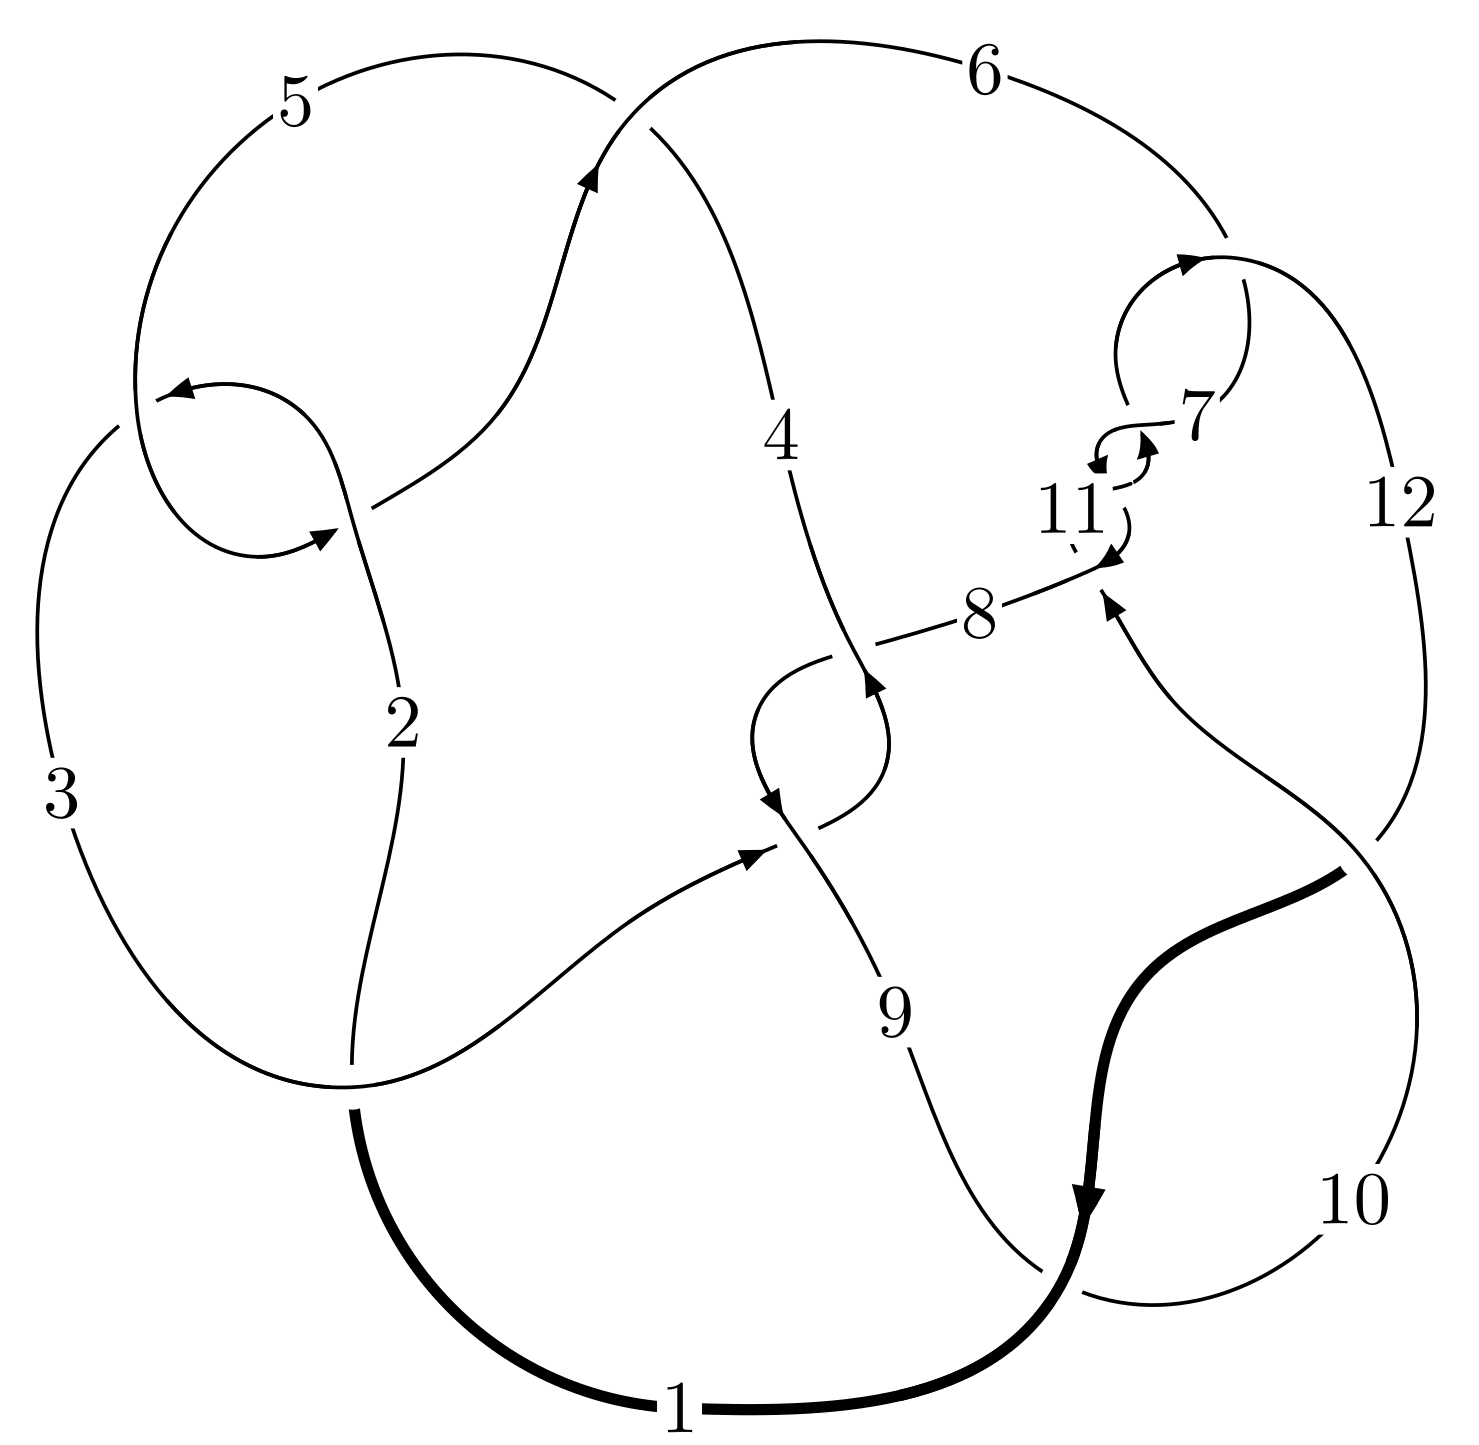
\includegraphics[width=112pt]{../../../GIT/diagram.site/Diagrams/png/984_12a_0183.png}\\
\ \ \ A knot diagram\footnotemark}&
\allowdisplaybreaks
\textbf{Linearized knot diagam} \\
\cline{2-2}
 &
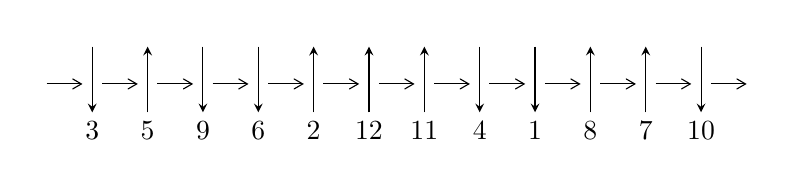
\begin{tikzpicture}[x=20pt, y=17pt]
	% nodes
	\node (C0) at (0, 0) {};
	\node (C1) at (1, 0) {};
	\node (C1U) at (1, +1) {};
	\node (C1D) at (1, -1) {3};

	\node (C2) at (2, 0) {};
	\node (C2U) at (2, +1) {};
	\node (C2D) at (2, -1) {5};

	\node (C3) at (3, 0) {};
	\node (C3U) at (3, +1) {};
	\node (C3D) at (3, -1) {9};

	\node (C4) at (4, 0) {};
	\node (C4U) at (4, +1) {};
	\node (C4D) at (4, -1) {6};

	\node (C5) at (5, 0) {};
	\node (C5U) at (5, +1) {};
	\node (C5D) at (5, -1) {2};

	\node (C6) at (6, 0) {};
	\node (C6U) at (6, +1) {};
	\node (C6D) at (6, -1) {12};

	\node (C7) at (7, 0) {};
	\node (C7U) at (7, +1) {};
	\node (C7D) at (7, -1) {11};

	\node (C8) at (8, 0) {};
	\node (C8U) at (8, +1) {};
	\node (C8D) at (8, -1) {4};

	\node (C9) at (9, 0) {};
	\node (C9U) at (9, +1) {};
	\node (C9D) at (9, -1) {1};

	\node (C10) at (10, 0) {};
	\node (C10U) at (10, +1) {};
	\node (C10D) at (10, -1) {8};

	\node (C11) at (11, 0) {};
	\node (C11U) at (11, +1) {};
	\node (C11D) at (11, -1) {7};

	\node (C12) at (12, 0) {};
	\node (C12U) at (12, +1) {};
	\node (C12D) at (12, -1) {10};
	\node (C13) at (13, 0) {};

	% arrows
	\draw[->,>={angle 60}]
	(C0) edge (C1) (C1) edge (C2) (C2) edge (C3) (C3) edge (C4) (C4) edge (C5) (C5) edge (C6) (C6) edge (C7) (C7) edge (C8) (C8) edge (C9) (C9) edge (C10) (C10) edge (C11) (C11) edge (C12) (C12) edge (C13) ;	\draw[->,>=stealth]
	(C1U) edge (C1D) (C2D) edge (C2U) (C3U) edge (C3D) (C4U) edge (C4D) (C5D) edge (C5U) (C6D) edge (C6U) (C7D) edge (C7U) (C8U) edge (C8D) (C9U) edge (C9D) (C10D) edge (C10U) (C11D) edge (C11U) (C12U) edge (C12D) ;
	\end{tikzpicture} \\
\hhline{~~} \\& 
\textbf{Solving Sequence} \\ \cline{2-2} 
 &
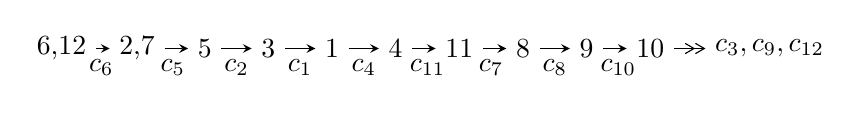
\begin{tikzpicture}[x=23pt, y=7pt]
	% node
	\node (A0) at (-1/8, 0) {6,12};
	\node (A1) at (17/16, 0) {2,7};
	\node (A2) at (17/8, 0) {5};
	\node (A3) at (25/8, 0) {3};
	\node (A4) at (33/8, 0) {1};
	\node (A5) at (41/8, 0) {4};
	\node (A6) at (49/8, 0) {11};
	\node (A7) at (57/8, 0) {8};
	\node (A8) at (65/8, 0) {9};
	\node (A9) at (73/8, 0) {10};
	\node (C1) at (1/2, -1) {$c_{6}$};
	\node (C2) at (13/8, -1) {$c_{5}$};
	\node (C3) at (21/8, -1) {$c_{2}$};
	\node (C4) at (29/8, -1) {$c_{1}$};
	\node (C5) at (37/8, -1) {$c_{4}$};
	\node (C6) at (45/8, -1) {$c_{11}$};
	\node (C7) at (53/8, -1) {$c_{7}$};
	\node (C8) at (61/8, -1) {$c_{8}$};
	\node (C9) at (69/8, -1) {$c_{10}$};
	\node (A10) at (11, 0) {$c_{3},c_{9},c_{12}$};

	% edge
	\draw[->,>=stealth]	
	(A0) edge (A1) (A1) edge (A2) (A2) edge (A3) (A3) edge (A4) (A4) edge (A5) (A5) edge (A6) (A6) edge (A7) (A7) edge (A8) (A8) edge (A9) ;
	\draw[->>,>={angle 60}]	
	(A9) edge (A10);
\end{tikzpicture} \\ 

\end{tabular} \\

\footnotetext{
The image of knot diagram is generated by the software ``\textbf{Draw programme}" developed by Andrew Bartholomew(\url{http://www.layer8.co.uk/maths/draw/index.htm\#Running-draw}), where we modified some parts for our purpose(\url{https://github.com/CATsTAILs/LinksPainter}).
}\phantom \\ \newline 
\centering \textbf{Ideals for irreducible components\footnotemark of $X_{\text{par}}$} 
 
\begin{align*}
I^u_{1}&=\langle 
- u^{67}-2 u^{66}+\cdots+2 b-6 u,\;- u^{67}-3 u^{66}+\cdots+2 a-4,\;u^{68}+3 u^{67}+\cdots+2 u+1\rangle \\
I^u_{2}&=\langle 
- u^3 a- u^3-3 a u+2 b- a-3 u-1,\;u^3 a+u^2 a+u^3+a^2+3 a u+3 a+2 u,\;u^4+u^3+3 u^2+2 u+1\rangle \\
\\
\end{align*}
\raggedright * 2 irreducible components of $\dim_{\mathbb{C}}=0$, with total 76 representations.\\
\footnotetext{All coefficients of polynomials are rational numbers. But the coefficients are sometimes approximated in decimal forms when there is not enough margin.}
\newpage
\renewcommand{\arraystretch}{1}
\centering \section*{I. $I^u_{1}= \langle - u^{67}-2 u^{66}+\cdots+2 b-6 u,\;- u^{67}-3 u^{66}+\cdots+2 a-4,\;u^{68}+3 u^{67}+\cdots+2 u+1 \rangle$}
\flushleft \textbf{(i) Arc colorings}\\
\begin{tabular}{m{7pt} m{180pt} m{7pt} m{180pt} }
\flushright $a_{6}=$&$\begin{pmatrix}1\\0\end{pmatrix}$ \\
\flushright $a_{12}=$&$\begin{pmatrix}0\\u\end{pmatrix}$ \\
\flushright $a_{2}=$&$\begin{pmatrix}\frac{1}{2} u^{67}+\frac{3}{2} u^{66}+\cdots-3 u+2\\\frac{1}{2} u^{67}+u^{66}+\cdots-5 u^2+3 u\end{pmatrix}$ \\
\flushright $a_{7}=$&$\begin{pmatrix}1\\- u^2\end{pmatrix}$ \\
\flushright $a_{5}=$&$\begin{pmatrix}u^{67}+\frac{5}{2} u^{66}+\cdots+6 u+4\\-\frac{1}{2} u^{67}-2 u^{66}+\cdots+u-2\end{pmatrix}$ \\
\flushright $a_{3}=$&$\begin{pmatrix}\frac{7}{2} u^{67}+\frac{17}{2} u^{66}+\cdots+11 u+5\\-\frac{3}{2} u^{67}-5 u^{66}+\cdots-37 u^2-3\end{pmatrix}$ \\
\flushright $a_{1}=$&$\begin{pmatrix}- u^7-4 u^5-4 u^3\\u^9+5 u^7+7 u^5+2 u^3+u\end{pmatrix}$ \\
\flushright $a_{4}=$&$\begin{pmatrix}\frac{1}{2} u^{67}+\frac{1}{2} u^{66}+\cdots+7 u+2\\-\frac{1}{2} u^{67}-2 u^{66}+\cdots+u-2\end{pmatrix}$ \\
\flushright $a_{11}=$&$\begin{pmatrix}- u\\u^3+u\end{pmatrix}$ \\
\flushright $a_{8}=$&$\begin{pmatrix}u^2+1\\- u^4-2 u^2\end{pmatrix}$ \\
\flushright $a_{9}=$&$\begin{pmatrix}u^{11}+6 u^9+12 u^7+8 u^5+u^3+2 u\\- u^{13}-7 u^{11}-17 u^9-16 u^7-6 u^5-5 u^3- u\end{pmatrix}$ \\
\flushright $a_{10}=$&$\begin{pmatrix}- u^3-2 u\\u^5+3 u^3+u\end{pmatrix}$\\&\end{tabular}
\flushleft \textbf{(ii) Obstruction class $= -1$}\\~\\
\flushleft \textbf{(iii) Cusp Shapes $= -\frac{11}{2} u^{67}-14 u^{66}+\cdots-29 u-\frac{11}{2}$}\\~\\
\newpage\renewcommand{\arraystretch}{1}
\flushleft \textbf{(iv) u-Polynomials at the component}\newline \\
\begin{tabular}{m{50pt}|m{274pt}}
Crossings & \hspace{64pt}u-Polynomials at each crossing \\
\hline $$\begin{aligned}c_{1},c_{4}\end{aligned}$$&$\begin{aligned}
&u^{68}+21 u^{67}+\cdots+34 u+1
\end{aligned}$\\
\hline $$\begin{aligned}c_{2},c_{5}\end{aligned}$$&$\begin{aligned}
&u^{68}+5 u^{67}+\cdots+17 u^2+1
\end{aligned}$\\
\hline $$\begin{aligned}c_{3},c_{8}\end{aligned}$$&$\begin{aligned}
&u^{68}+u^{67}+\cdots+640 u+256
\end{aligned}$\\
\hline $$\begin{aligned}c_{6},c_{7},c_{10}\\c_{11}\end{aligned}$$&$\begin{aligned}
&u^{68}+3 u^{67}+\cdots+2 u+1
\end{aligned}$\\
\hline $$\begin{aligned}c_{9},c_{12}\end{aligned}$$&$\begin{aligned}
&u^{68}-11 u^{67}+\cdots+328 u+209
\end{aligned}$\\
\hline
\end{tabular}\\~\\
\newpage\renewcommand{\arraystretch}{1}
\flushleft \textbf{(v) Riley Polynomials at the component}\newline \\
\begin{tabular}{m{50pt}|m{274pt}}
Crossings & \hspace{64pt}Riley Polynomials at each crossing \\
\hline $$\begin{aligned}c_{1},c_{4}\end{aligned}$$&$\begin{aligned}
&y^{68}+57 y^{67}+\cdots+2 y+1
\end{aligned}$\\
\hline $$\begin{aligned}c_{2},c_{5}\end{aligned}$$&$\begin{aligned}
&y^{68}+21 y^{67}+\cdots+34 y+1
\end{aligned}$\\
\hline $$\begin{aligned}c_{3},c_{8}\end{aligned}$$&$\begin{aligned}
&y^{68}+45 y^{67}+\cdots+606208 y+65536
\end{aligned}$\\
\hline $$\begin{aligned}c_{6},c_{7},c_{10}\\c_{11}\end{aligned}$$&$\begin{aligned}
&y^{68}+75 y^{67}+\cdots+26 y+1
\end{aligned}$\\
\hline $$\begin{aligned}c_{9},c_{12}\end{aligned}$$&$\begin{aligned}
&y^{68}+51 y^{67}+\cdots+1645090 y+43681
\end{aligned}$\\
\hline
\end{tabular}\\~\\
\newpage\flushleft \textbf{(vi) Complex Volumes and Cusp Shapes}
$$\begin{array}{c|c|c}  
\text{Solutions to }I^u_{1}& \I (\text{vol} + \sqrt{-1}CS) & \text{Cusp shape}\\
 \hline 
\begin{aligned}
u &= \phantom{-}0.302515 + 0.808830 I \\
a &= \phantom{-}1.38035 - 1.18783 I \\
b &= -0.748496 - 0.927452 I\end{aligned}
 & \phantom{-}2.32422 + 5.97645 I & \phantom{-0.000000 } 0. - 7.23199 I \\ \hline\begin{aligned}
u &= \phantom{-}0.302515 - 0.808830 I \\
a &= \phantom{-}1.38035 + 1.18783 I \\
b &= -0.748496 + 0.927452 I\end{aligned}
 & \phantom{-}2.32422 - 5.97645 I & \phantom{-0.000000 -}0. + 7.23199 I \\ \hline\begin{aligned}
u &= -0.624582 + 0.592516 I \\
a &= \phantom{-}2.73939 + 0.45090 I \\
b &= -0.782644 + 1.029050 I\end{aligned}
 & \phantom{-}8.5059 - 11.6125 I & \phantom{-0.000000 -}0. + 8.82159 I \\ \hline\begin{aligned}
u &= -0.624582 - 0.592516 I \\
a &= \phantom{-}2.73939 - 0.45090 I \\
b &= -0.782644 - 1.029050 I\end{aligned}
 & \phantom{-}8.5059 + 11.6125 I & \phantom{-0.000000 } 0. - 8.82159 I \\ \hline\begin{aligned}
u &= -0.631706 + 0.575663 I \\
a &= \phantom{-}0.66472 + 1.66346 I \\
b &= -0.898485 - 0.736878 I\end{aligned}
 & \phantom{-}9.41750 - 5.39141 I & \phantom{-}4.69572 + 4.02325 I \\ \hline\begin{aligned}
u &= -0.631706 - 0.575663 I \\
a &= \phantom{-}0.66472 - 1.66346 I \\
b &= -0.898485 + 0.736878 I\end{aligned}
 & \phantom{-}9.41750 + 5.39141 I & \phantom{-}4.69572 - 4.02325 I \\ \hline\begin{aligned}
u &= \phantom{-}0.346423 + 0.771113 I \\
a &= -0.173545 - 0.361476 I \\
b &= -0.764235 + 0.828111 I\end{aligned}
 & \phantom{-}2.62914 + 0.24601 I & \phantom{-0.000000 } 0. - 1.73579 I \\ \hline\begin{aligned}
u &= \phantom{-}0.346423 - 0.771113 I \\
a &= -0.173545 + 0.361476 I \\
b &= -0.764235 - 0.828111 I\end{aligned}
 & \phantom{-}2.62914 - 0.24601 I & \phantom{-0.000000 -}0. + 1.73579 I \\ \hline\begin{aligned}
u &= -0.573633 + 0.539020 I \\
a &= -1.74644 - 0.39374 I \\
b &= \phantom{-}0.275978 - 1.117340 I\end{aligned}
 & \phantom{-}1.46789 - 5.68286 I & \phantom{-}0.68260 + 7.74797 I \\ \hline\begin{aligned}
u &= -0.573633 - 0.539020 I \\
a &= -1.74644 + 0.39374 I \\
b &= \phantom{-}0.275978 + 1.117340 I\end{aligned}
 & \phantom{-}1.46789 + 5.68286 I & \phantom{-}0.68260 - 7.74797 I\\
 \hline 
 \end{array}$$\newpage$$\begin{array}{c|c|c}  
\text{Solutions to }I^u_{1}& \I (\text{vol} + \sqrt{-1}CS) & \text{Cusp shape}\\
 \hline 
\begin{aligned}
u &= \phantom{-}0.598138 + 0.510537 I \\
a &= -2.96024 - 0.40706 I \\
b &= \phantom{-}0.768075 + 0.897553 I\end{aligned}
 & \phantom{-}4.42265 + 4.95521 I & \phantom{-}3.07955 - 6.13595 I \\ \hline\begin{aligned}
u &= \phantom{-}0.598138 - 0.510537 I \\
a &= -2.96024 + 0.40706 I \\
b &= \phantom{-}0.768075 - 0.897553 I\end{aligned}
 & \phantom{-}4.42265 - 4.95521 I & \phantom{-}3.07955 + 6.13595 I \\ \hline\begin{aligned}
u &= -0.663956 + 0.416976 I \\
a &= \phantom{-}1.98971 - 0.58484 I \\
b &= -0.894047 + 0.760345 I\end{aligned}
 & \phantom{-}9.88771 + 1.02189 I & \phantom{-}5.85214 + 1.96232 I \\ \hline\begin{aligned}
u &= -0.663956 - 0.416976 I \\
a &= \phantom{-}1.98971 + 0.58484 I \\
b &= -0.894047 - 0.760345 I\end{aligned}
 & \phantom{-}9.88771 - 1.02189 I & \phantom{-}5.85214 - 1.96232 I \\ \hline\begin{aligned}
u &= -0.607629 + 0.495214 I \\
a &= -1.199490 - 0.617485 I \\
b &= \phantom{-}0.803603 - 0.027754 I\end{aligned}
 & \phantom{-}5.30813 - 2.06794 I & \phantom{-}6.26189 + 3.47855 I \\ \hline\begin{aligned}
u &= -0.607629 - 0.495214 I \\
a &= -1.199490 + 0.617485 I \\
b &= \phantom{-}0.803603 + 0.027754 I\end{aligned}
 & \phantom{-}5.30813 + 2.06794 I & \phantom{-}6.26189 - 3.47855 I \\ \hline\begin{aligned}
u &= -0.664613 + 0.394825 I \\
a &= \phantom{-}1.54657 + 1.01878 I \\
b &= -0.792225 - 1.015100 I\end{aligned}
 & \phantom{-}9.09143 + 7.26370 I & \phantom{-}4.68955 - 2.96843 I \\ \hline\begin{aligned}
u &= -0.664613 - 0.394825 I \\
a &= \phantom{-}1.54657 - 1.01878 I \\
b &= -0.792225 + 1.015100 I\end{aligned}
 & \phantom{-}9.09143 - 7.26370 I & \phantom{-}4.68955 + 2.96843 I \\ \hline\begin{aligned}
u &= \phantom{-}0.601390 + 0.478255 I \\
a &= -1.47390 + 1.84744 I \\
b &= \phantom{-}0.774996 - 0.866635 I\end{aligned}
 & \phantom{-}4.51797 - 0.86560 I & \phantom{-}3.52173 - 0.59232 I \\ \hline\begin{aligned}
u &= \phantom{-}0.601390 - 0.478255 I \\
a &= -1.47390 - 1.84744 I \\
b &= \phantom{-}0.774996 + 0.866635 I\end{aligned}
 & \phantom{-}4.51797 + 0.86560 I & \phantom{-}3.52173 + 0.59232 I\\
 \hline 
 \end{array}$$\newpage$$\begin{array}{c|c|c}  
\text{Solutions to }I^u_{1}& \I (\text{vol} + \sqrt{-1}CS) & \text{Cusp shape}\\
 \hline 
\begin{aligned}
u &= \phantom{-}0.468377 + 0.572220 I \\
a &= \phantom{-}1.90643 - 0.33431 I \\
b &= -0.122342 - 0.726340 I\end{aligned}
 & -0.59228 + 2.22769 I & -3.37234 - 3.06639 I \\ \hline\begin{aligned}
u &= \phantom{-}0.468377 - 0.572220 I \\
a &= \phantom{-}1.90643 + 0.33431 I \\
b &= -0.122342 + 0.726340 I\end{aligned}
 & -0.59228 - 2.22769 I & -3.37234 + 3.06639 I \\ \hline\begin{aligned}
u &= -0.576072 + 0.442170 I \\
a &= \phantom{-}0.006747 - 0.329071 I \\
b &= \phantom{-}0.319410 + 1.099330 I\end{aligned}
 & \phantom{-}1.75394 + 1.73798 I & \phantom{-}2.20480 - 0.79061 I \\ \hline\begin{aligned}
u &= -0.576072 - 0.442170 I \\
a &= \phantom{-}0.006747 + 0.329071 I \\
b &= \phantom{-}0.319410 - 1.099330 I\end{aligned}
 & \phantom{-}1.75394 - 1.73798 I & \phantom{-}2.20480 + 0.79061 I \\ \hline\begin{aligned}
u &= \phantom{-}0.092300 + 0.677316 I \\
a &= \phantom{-}0.27605 + 1.89597 I \\
b &= \phantom{-}0.128373 + 0.916246 I\end{aligned}
 & -2.81890 + 1.99447 I & -8.57513 - 4.98912 I \\ \hline\begin{aligned}
u &= \phantom{-}0.092300 - 0.677316 I \\
a &= \phantom{-}0.27605 - 1.89597 I \\
b &= \phantom{-}0.128373 - 0.916246 I\end{aligned}
 & -2.81890 - 1.99447 I & -8.57513 + 4.98912 I \\ \hline\begin{aligned}
u &= \phantom{-}0.587653 + 0.024788 I \\
a &= \phantom{-}1.71449 + 0.76043 I \\
b &= -0.778469 - 0.883411 I\end{aligned}
 & \phantom{-}4.96906 + 2.93148 I & \phantom{-}6.24702 - 2.99694 I \\ \hline\begin{aligned}
u &= \phantom{-}0.587653 - 0.024788 I \\
a &= \phantom{-}1.71449 - 0.76043 I \\
b &= -0.778469 + 0.883411 I\end{aligned}
 & \phantom{-}4.96906 - 2.93148 I & \phantom{-}6.24702 + 2.99694 I \\ \hline\begin{aligned}
u &= -0.18308 + 1.42922 I \\
a &= \phantom{-}0.843168 + 0.142200 I \\
b &= -0.806444 - 0.993390 I\end{aligned}
 & \phantom{-}3.26662 + 4.24372 I & \phantom{-0.000000 } 0 \\ \hline\begin{aligned}
u &= -0.18308 - 1.42922 I \\
a &= \phantom{-}0.843168 - 0.142200 I \\
b &= -0.806444 + 0.993390 I\end{aligned}
 & \phantom{-}3.26662 - 4.24372 I & \phantom{-0.000000 } 0\\
 \hline 
 \end{array}$$\newpage$$\begin{array}{c|c|c}  
\text{Solutions to }I^u_{1}& \I (\text{vol} + \sqrt{-1}CS) & \text{Cusp shape}\\
 \hline 
\begin{aligned}
u &= -0.19116 + 1.44793 I \\
a &= \phantom{-}1.213650 + 0.087479 I \\
b &= -0.888277 + 0.792353 I\end{aligned}
 & \phantom{-}3.89634 - 2.02780 I & \phantom{-0.000000 } 0 \\ \hline\begin{aligned}
u &= -0.19116 - 1.44793 I \\
a &= \phantom{-}1.213650 - 0.087479 I \\
b &= -0.888277 - 0.792353 I\end{aligned}
 & \phantom{-}3.89634 + 2.02780 I & \phantom{-0.000000 } 0 \\ \hline\begin{aligned}
u &= \phantom{-}0.394466 + 0.343618 I \\
a &= \phantom{-}0.574285 - 0.334716 I \\
b &= \phantom{-}0.015724 + 0.516322 I\end{aligned}
 & \phantom{-}0.058562 + 0.963973 I & \phantom{-}0.65757 - 5.10087 I \\ \hline\begin{aligned}
u &= \phantom{-}0.394466 - 0.343618 I \\
a &= \phantom{-}0.574285 + 0.334716 I \\
b &= \phantom{-}0.015724 - 0.516322 I\end{aligned}
 & \phantom{-}0.058562 - 0.963973 I & \phantom{-}0.65757 + 5.10087 I \\ \hline\begin{aligned}
u &= -0.143999 + 0.479957 I \\
a &= -2.56050 - 1.66131 I \\
b &= \phantom{-}0.567438 - 0.923967 I\end{aligned}
 & -0.46907 - 2.83971 I & -5.96216 + 1.53375 I \\ \hline\begin{aligned}
u &= -0.143999 - 0.479957 I \\
a &= -2.56050 + 1.66131 I \\
b &= \phantom{-}0.567438 + 0.923967 I\end{aligned}
 & -0.46907 + 2.83971 I & -5.96216 - 1.53375 I \\ \hline\begin{aligned}
u &= \phantom{-}0.00733 + 1.50712 I \\
a &= \phantom{-}0.012768 - 0.380965 I \\
b &= \phantom{-}0.636378 + 0.533093 I\end{aligned}
 & -5.97370 + 1.45056 I & \phantom{-0.000000 } 0 \\ \hline\begin{aligned}
u &= \phantom{-}0.00733 - 1.50712 I \\
a &= \phantom{-}0.012768 + 0.380965 I \\
b &= \phantom{-}0.636378 - 0.533093 I\end{aligned}
 & -5.97370 - 1.45056 I & \phantom{-0.000000 } 0 \\ \hline\begin{aligned}
u &= -0.14976 + 1.50240 I \\
a &= \phantom{-}0.124282 + 0.756614 I \\
b &= \phantom{-}0.375721 + 1.104200 I\end{aligned}
 & -4.62766 - 0.77309 I & \phantom{-0.000000 } 0 \\ \hline\begin{aligned}
u &= -0.14976 - 1.50240 I \\
a &= \phantom{-}0.124282 - 0.756614 I \\
b &= \phantom{-}0.375721 - 1.104200 I\end{aligned}
 & -4.62766 + 0.77309 I & \phantom{-0.000000 } 0\\
 \hline 
 \end{array}$$\newpage$$\begin{array}{c|c|c}  
\text{Solutions to }I^u_{1}& \I (\text{vol} + \sqrt{-1}CS) & \text{Cusp shape}\\
 \hline 
\begin{aligned}
u &= \phantom{-}0.17091 + 1.50831 I \\
a &= -0.738203 + 1.030050 I \\
b &= \phantom{-}0.789562 - 0.833836 I\end{aligned}
 & -2.00478 + 1.87390 I & \phantom{-0.000000 } 0 \\ \hline\begin{aligned}
u &= \phantom{-}0.17091 - 1.50831 I \\
a &= -0.738203 - 1.030050 I \\
b &= \phantom{-}0.789562 + 0.833836 I\end{aligned}
 & -2.00478 - 1.87390 I & \phantom{-0.000000 } 0 \\ \hline\begin{aligned}
u &= \phantom{-}0.299638 + 0.369423 I \\
a &= \phantom{-}0.473108 - 0.124443 I \\
b &= \phantom{-}0.122349 + 0.323173 I\end{aligned}
 & \phantom{-}0.065320 + 0.982452 I & \phantom{-}1.03774 - 6.49318 I \\ \hline\begin{aligned}
u &= \phantom{-}0.299638 - 0.369423 I \\
a &= \phantom{-}0.473108 + 0.124443 I \\
b &= \phantom{-}0.122349 - 0.323173 I\end{aligned}
 & \phantom{-}0.065320 - 0.982452 I & \phantom{-}1.03774 + 6.49318 I \\ \hline\begin{aligned}
u &= -0.17745 + 1.51476 I \\
a &= -0.500515 - 0.516152 I \\
b &= \phantom{-}0.814781 - 0.083742 I\end{aligned}
 & -1.30179 - 4.87223 I & \phantom{-0.000000 } 0 \\ \hline\begin{aligned}
u &= -0.17745 - 1.51476 I \\
a &= -0.500515 + 0.516152 I \\
b &= \phantom{-}0.814781 + 0.083742 I\end{aligned}
 & -1.30179 + 4.87223 I & \phantom{-0.000000 } 0 \\ \hline\begin{aligned}
u &= \phantom{-}0.08984 + 1.52674 I \\
a &= \phantom{-}0.591800 + 0.051249 I \\
b &= -0.313816 + 0.326902 I\end{aligned}
 & -6.47425 + 2.47932 I & \phantom{-0.000000 } 0 \\ \hline\begin{aligned}
u &= \phantom{-}0.08984 - 1.52674 I \\
a &= \phantom{-}0.591800 - 0.051249 I \\
b &= -0.313816 - 0.326902 I\end{aligned}
 & -6.47425 - 2.47932 I & \phantom{-0.000000 } 0 \\ \hline\begin{aligned}
u &= -0.02436 + 1.53342 I \\
a &= -1.32376 - 1.50760 I \\
b &= \phantom{-}0.589779 - 0.999381 I\end{aligned}
 & -7.31420 - 3.34180 I & \phantom{-0.000000 } 0 \\ \hline\begin{aligned}
u &= -0.02436 - 1.53342 I \\
a &= -1.32376 + 1.50760 I \\
b &= \phantom{-}0.589779 + 0.999381 I\end{aligned}
 & -7.31420 + 3.34180 I & \phantom{-0.000000 } 0\\
 \hline 
 \end{array}$$\newpage$$\begin{array}{c|c|c}  
\text{Solutions to }I^u_{1}& \I (\text{vol} + \sqrt{-1}CS) & \text{Cusp shape}\\
 \hline 
\begin{aligned}
u &= \phantom{-}0.17598 + 1.52392 I \\
a &= -2.15557 + 0.42536 I \\
b &= \phantom{-}0.765471 + 0.926847 I\end{aligned}
 & -2.29162 + 7.72916 I & \phantom{-0.000000 } 0 \\ \hline\begin{aligned}
u &= \phantom{-}0.17598 - 1.52392 I \\
a &= -2.15557 - 0.42536 I \\
b &= \phantom{-}0.765471 - 0.926847 I\end{aligned}
 & -2.29162 - 7.72916 I & \phantom{-0.000000 } 0 \\ \hline\begin{aligned}
u &= -0.17029 + 1.53953 I \\
a &= -1.21280 - 1.29053 I \\
b &= \phantom{-}0.245144 - 1.137840 I\end{aligned}
 & -5.43631 - 8.36637 I & \phantom{-0.000000 } 0 \\ \hline\begin{aligned}
u &= -0.17029 - 1.53953 I \\
a &= -1.21280 + 1.29053 I \\
b &= \phantom{-}0.245144 + 1.137840 I\end{aligned}
 & -5.43631 + 8.36637 I & \phantom{-0.000000 } 0 \\ \hline\begin{aligned}
u &= -0.19769 + 1.55029 I \\
a &= \phantom{-}0.060610 + 0.906239 I \\
b &= -0.901287 - 0.714793 I\end{aligned}
 & \phantom{-}2.37596 - 8.42534 I & \phantom{-0.000000 } 0 \\ \hline\begin{aligned}
u &= -0.19769 - 1.55029 I \\
a &= \phantom{-}0.060610 - 0.906239 I \\
b &= -0.901287 + 0.714793 I\end{aligned}
 & \phantom{-}2.37596 + 8.42534 I & \phantom{-0.000000 } 0 \\ \hline\begin{aligned}
u &= \phantom{-}0.13226 + 1.55786 I \\
a &= \phantom{-}1.43128 - 1.00095 I \\
b &= -0.168861 - 0.801656 I\end{aligned}
 & -7.75675 + 4.39339 I & \phantom{-0.000000 } 0 \\ \hline\begin{aligned}
u &= \phantom{-}0.13226 - 1.55786 I \\
a &= \phantom{-}1.43128 + 1.00095 I \\
b &= -0.168861 + 0.801656 I\end{aligned}
 & -7.75675 - 4.39339 I & \phantom{-0.000000 } 0 \\ \hline\begin{aligned}
u &= -0.19499 + 1.55859 I \\
a &= \phantom{-}1.91320 + 1.14117 I \\
b &= -0.773177 + 1.040270 I\end{aligned}
 & \phantom{-}1.3625 - 14.6199 I & \phantom{-0.000000 } 0 \\ \hline\begin{aligned}
u &= -0.19499 - 1.55859 I \\
a &= \phantom{-}1.91320 - 1.14117 I \\
b &= -0.773177 - 1.040270 I\end{aligned}
 & \phantom{-}1.3625 + 14.6199 I & \phantom{-0.000000 } 0\\
 \hline 
 \end{array}$$\newpage$$\begin{array}{c|c|c}  
\text{Solutions to }I^u_{1}& \I (\text{vol} + \sqrt{-1}CS) & \text{Cusp shape}\\
 \hline 
\begin{aligned}
u &= \phantom{-}0.02362 + 1.57367 I \\
a &= \phantom{-}0.27679 + 1.90830 I \\
b &= \phantom{-}0.061066 + 0.995702 I\end{aligned}
 & -10.44290 + 2.40599 I & \phantom{-0.000000 } 0 \\ \hline\begin{aligned}
u &= \phantom{-}0.02362 - 1.57367 I \\
a &= \phantom{-}0.27679 - 1.90830 I \\
b &= \phantom{-}0.061066 - 0.995702 I\end{aligned}
 & -10.44290 - 2.40599 I & \phantom{-0.000000 } 0 \\ \hline\begin{aligned}
u &= \phantom{-}0.08488 + 1.60162 I \\
a &= -0.205262 + 0.369099 I \\
b &= -0.719407 + 0.791988 I\end{aligned}
 & -5.42283 + 1.77686 I & \phantom{-0.000000 } 0 \\ \hline\begin{aligned}
u &= \phantom{-}0.08488 - 1.60162 I \\
a &= -0.205262 - 0.369099 I \\
b &= -0.719407 - 0.791988 I\end{aligned}
 & -5.42283 - 1.77686 I & \phantom{-0.000000 } 0 \\ \hline\begin{aligned}
u &= \phantom{-}0.06715 + 1.60931 I \\
a &= \phantom{-}0.72881 - 1.41338 I \\
b &= -0.709021 - 0.945322 I\end{aligned}
 & -5.89990 + 7.25511 I & \phantom{-0.000000 } 0 \\ \hline\begin{aligned}
u &= \phantom{-}0.06715 - 1.60931 I \\
a &= \phantom{-}0.72881 + 1.41338 I \\
b &= -0.709021 + 0.945322 I\end{aligned}
 & -5.89990 - 7.25511 I & \phantom{-0.000000 } 0 \\ \hline\begin{aligned}
u &= -0.167888 + 0.269376 I \\
a &= \phantom{-}0.78201 - 2.05483 I \\
b &= \phantom{-}0.507386 + 0.771126 I\end{aligned}
 & \phantom{-}0.08583 + 1.52615 I & -2.20733 - 5.34922 I \\ \hline\begin{aligned}
u &= -0.167888 - 0.269376 I \\
a &= \phantom{-}0.78201 + 2.05483 I \\
b &= \phantom{-}0.507386 - 0.771126 I\end{aligned}
 & \phantom{-}0.08583 - 1.52615 I & -2.20733 + 5.34922 I\\
 \hline 
 \end{array}$$\newpage\newpage\renewcommand{\arraystretch}{1}
\centering \section*{II. $I^u_{2}= \langle - u^3 a- u^3-3 a u+2 b- a-3 u-1,\;u^3 a+u^2 a+u^3+a^2+3 a u+3 a+2 u,\;u^4+u^3+3 u^2+2 u+1 \rangle$}
\flushleft \textbf{(i) Arc colorings}\\
\begin{tabular}{m{7pt} m{180pt} m{7pt} m{180pt} }
\flushright $a_{6}=$&$\begin{pmatrix}1\\0\end{pmatrix}$ \\
\flushright $a_{12}=$&$\begin{pmatrix}0\\u\end{pmatrix}$ \\
\flushright $a_{2}=$&$\begin{pmatrix}a\\\frac{1}{2} u^3 a+\frac{1}{2} u^3+\cdots+\frac{1}{2} a+\frac{1}{2}\end{pmatrix}$ \\
\flushright $a_{7}=$&$\begin{pmatrix}1\\- u^2\end{pmatrix}$ \\
\flushright $a_{5}=$&$\begin{pmatrix}-\frac{1}{2} u^3 a+\frac{1}{2} u^3+\cdots+\frac{1}{2} a+\frac{5}{2}\\\frac{1}{2} u^3 a+\frac{1}{2} u^3+\cdots+\frac{1}{2} a-\frac{1}{2}\end{pmatrix}$ \\
\flushright $a_{3}=$&$\begin{pmatrix}u^3+u^2+a+3 u+2\\\frac{1}{2} u^3 a+\frac{1}{2} u^3+\cdots+\frac{1}{2} a-\frac{1}{2}\end{pmatrix}$ \\
\flushright $a_{1}=$&$\begin{pmatrix}-1\\0\end{pmatrix}$ \\
\flushright $a_{4}=$&$\begin{pmatrix}u^3+u^2+a+3 u+2\\\frac{1}{2} u^3 a+\frac{1}{2} u^3+\cdots+\frac{1}{2} a-\frac{1}{2}\end{pmatrix}$ \\
\flushright $a_{11}=$&$\begin{pmatrix}- u\\u^3+u\end{pmatrix}$ \\
\flushright $a_{8}=$&$\begin{pmatrix}u^2+1\\u^3+u^2+2 u+1\end{pmatrix}$ \\
\flushright $a_{9}=$&$\begin{pmatrix}u^2+1\\u^3+u^2+2 u+1\end{pmatrix}$ \\
\flushright $a_{10}=$&$\begin{pmatrix}- u^3-2 u\\u^3+u^2+2 u+1\end{pmatrix}$\\&\end{tabular}
\flushleft \textbf{(ii) Obstruction class $= 1$}\\~\\
\flushleft \textbf{(iii) Cusp Shapes $= -2 u^3 a+2 u^3-5 a u+4 u^2-3 a+6 u+3$}\\~\\
\newpage\renewcommand{\arraystretch}{1}
\flushleft \textbf{(iv) u-Polynomials at the component}\newline \\
\begin{tabular}{m{50pt}|m{274pt}}
Crossings & \hspace{64pt}u-Polynomials at each crossing \\
\hline $$\begin{aligned}c_{1},c_{4},c_{5}\end{aligned}$$&$\begin{aligned}
&(u^2- u+1)^4
\end{aligned}$\\
\hline $$\begin{aligned}c_{2}\end{aligned}$$&$\begin{aligned}
&(u^2+u+1)^4
\end{aligned}$\\
\hline $$\begin{aligned}c_{3},c_{8}\end{aligned}$$&$\begin{aligned}
&u^8
\end{aligned}$\\
\hline $$\begin{aligned}c_{6},c_{7}\end{aligned}$$&$\begin{aligned}
&(u^4+u^3+3 u^2+2 u+1)^2
\end{aligned}$\\
\hline $$\begin{aligned}c_{9}\end{aligned}$$&$\begin{aligned}
&(u^4+u^3+u^2+1)^2
\end{aligned}$\\
\hline $$\begin{aligned}c_{10},c_{11}\end{aligned}$$&$\begin{aligned}
&(u^4- u^3+3 u^2-2 u+1)^2
\end{aligned}$\\
\hline $$\begin{aligned}c_{12}\end{aligned}$$&$\begin{aligned}
&(u^4- u^3+u^2+1)^2
\end{aligned}$\\
\hline
\end{tabular}\\~\\
\newpage\renewcommand{\arraystretch}{1}
\flushleft \textbf{(v) Riley Polynomials at the component}\newline \\
\begin{tabular}{m{50pt}|m{274pt}}
Crossings & \hspace{64pt}Riley Polynomials at each crossing \\
\hline $$\begin{aligned}c_{1},c_{2},c_{4}\\c_{5}\end{aligned}$$&$\begin{aligned}
&(y^2+y+1)^4
\end{aligned}$\\
\hline $$\begin{aligned}c_{3},c_{8}\end{aligned}$$&$\begin{aligned}
&y^8
\end{aligned}$\\
\hline $$\begin{aligned}c_{6},c_{7},c_{10}\\c_{11}\end{aligned}$$&$\begin{aligned}
&(y^4+5 y^3+7 y^2+2 y+1)^2
\end{aligned}$\\
\hline $$\begin{aligned}c_{9},c_{12}\end{aligned}$$&$\begin{aligned}
&(y^4+y^3+3 y^2+2 y+1)^2
\end{aligned}$\\
\hline
\end{tabular}\\~\\
\newpage\flushleft \textbf{(vi) Complex Volumes and Cusp Shapes}
$$\begin{array}{c|c|c}  
\text{Solutions to }I^u_{2}& \I (\text{vol} + \sqrt{-1}CS) & \text{Cusp shape}\\
 \hline 
\begin{aligned}
u &= -0.395123 + 0.506844 I \\
a &= \phantom{-}0.084432 - 0.576081 I \\
b &= \phantom{-}0.500000 + 0.866025 I\end{aligned}
 & \phantom{-}0.211005 + 0.614778 I & -0.99907 + 2.29114 I \\ \hline\begin{aligned}
u &= -0.395123 + 0.506844 I \\
a &= -2.04112 - 0.65111 I \\
b &= \phantom{-}0.500000 - 0.866025 I\end{aligned}
 & \phantom{-}0.21101 - 3.44499 I & \phantom{-}2.00436 + 8.24669 I \\ \hline\begin{aligned}
u &= -0.395123 - 0.506844 I \\
a &= \phantom{-}0.084432 + 0.576081 I \\
b &= \phantom{-}0.500000 - 0.866025 I\end{aligned}
 & \phantom{-}0.211005 - 0.614778 I & -0.99907 - 2.29114 I \\ \hline\begin{aligned}
u &= -0.395123 - 0.506844 I \\
a &= -2.04112 + 0.65111 I \\
b &= \phantom{-}0.500000 + 0.866025 I\end{aligned}
 & \phantom{-}0.21101 + 3.44499 I & \phantom{-}2.00436 - 8.24669 I \\ \hline\begin{aligned}
u &= -0.10488 + 1.55249 I \\
a &= \phantom{-}0.033637 + 0.507913 I \\
b &= \phantom{-}0.500000 + 0.866025 I\end{aligned}
 & -6.79074 - 1.13408 I & -5.65243 - 1.40826 I \\ \hline\begin{aligned}
u &= -0.10488 + 1.55249 I \\
a &= -1.07695 - 1.14911 I \\
b &= \phantom{-}0.500000 - 0.866025 I\end{aligned}
 & -6.79074 - 5.19385 I & -1.85285 + 5.62657 I \\ \hline\begin{aligned}
u &= -0.10488 - 1.55249 I \\
a &= \phantom{-}0.033637 - 0.507913 I \\
b &= \phantom{-}0.500000 - 0.866025 I\end{aligned}
 & -6.79074 + 1.13408 I & -5.65243 + 1.40826 I \\ \hline\begin{aligned}
u &= -0.10488 - 1.55249 I \\
a &= -1.07695 + 1.14911 I \\
b &= \phantom{-}0.500000 + 0.866025 I\end{aligned}
 & -6.79074 + 5.19385 I & -1.85285 - 5.62657 I\\
 \hline 
 \end{array}$$\newpage
\newpage\renewcommand{\arraystretch}{1}
\centering \section*{ III. u-Polynomials}
\begin{tabular}{m{50pt}|m{274pt}}
Crossings & \hspace{64pt}u-Polynomials at each crossing \\
\hline $$\begin{aligned}c_{1},c_{4}\end{aligned}$$&$\begin{aligned}
&((u^2- u+1)^4)(u^{68}+21 u^{67}+\cdots+34 u+1)
\end{aligned}$\\
\hline $$\begin{aligned}c_{2}\end{aligned}$$&$\begin{aligned}
&((u^2+u+1)^4)(u^{68}+5 u^{67}+\cdots+17 u^2+1)
\end{aligned}$\\
\hline $$\begin{aligned}c_{3},c_{8}\end{aligned}$$&$\begin{aligned}
&u^8(u^{68}+u^{67}+\cdots+640 u+256)
\end{aligned}$\\
\hline $$\begin{aligned}c_{5}\end{aligned}$$&$\begin{aligned}
&((u^2- u+1)^4)(u^{68}+5 u^{67}+\cdots+17 u^2+1)
\end{aligned}$\\
\hline $$\begin{aligned}c_{6},c_{7}\end{aligned}$$&$\begin{aligned}
&((u^4+u^3+3 u^2+2 u+1)^2)(u^{68}+3 u^{67}+\cdots+2 u+1)
\end{aligned}$\\
\hline $$\begin{aligned}c_{9}\end{aligned}$$&$\begin{aligned}
&((u^4+u^3+u^2+1)^2)(u^{68}-11 u^{67}+\cdots+328 u+209)
\end{aligned}$\\
\hline $$\begin{aligned}c_{10},c_{11}\end{aligned}$$&$\begin{aligned}
&((u^4- u^3+3 u^2-2 u+1)^2)(u^{68}+3 u^{67}+\cdots+2 u+1)
\end{aligned}$\\
\hline $$\begin{aligned}c_{12}\end{aligned}$$&$\begin{aligned}
&((u^4- u^3+u^2+1)^2)(u^{68}-11 u^{67}+\cdots+328 u+209)
\end{aligned}$\\
\hline
\end{tabular}\newpage\renewcommand{\arraystretch}{1}
\centering \section*{ IV. Riley Polynomials}
\begin{tabular}{m{50pt}|m{274pt}}
Crossings & \hspace{64pt}Riley Polynomials at each crossing \\
\hline $$\begin{aligned}c_{1},c_{4}\end{aligned}$$&$\begin{aligned}
&((y^2+y+1)^4)(y^{68}+57 y^{67}+\cdots+2 y+1)
\end{aligned}$\\
\hline $$\begin{aligned}c_{2},c_{5}\end{aligned}$$&$\begin{aligned}
&((y^2+y+1)^4)(y^{68}+21 y^{67}+\cdots+34 y+1)
\end{aligned}$\\
\hline $$\begin{aligned}c_{3},c_{8}\end{aligned}$$&$\begin{aligned}
&y^8(y^{68}+45 y^{67}+\cdots+606208 y+65536)
\end{aligned}$\\
\hline $$\begin{aligned}c_{6},c_{7},c_{10}\\c_{11}\end{aligned}$$&$\begin{aligned}
&((y^4+5 y^3+7 y^2+2 y+1)^2)(y^{68}+75 y^{67}+\cdots+26 y+1)
\end{aligned}$\\
\hline $$\begin{aligned}c_{9},c_{12}\end{aligned}$$&$\begin{aligned}
&((y^4+y^3+3 y^2+2 y+1)^2)(y^{68}+51 y^{67}+\cdots+1645090 y+43681)
\end{aligned}$\\
\hline
\end{tabular}
\vskip 2pc
\end{document}